\documentclass[aspectratio=169,10pt]{beamer}

\usetheme{Madrid}
\usecolortheme{seahorse}
\usepackage{amsmath, amssymb, amsfonts}
\usepackage{graphicx}
\usepackage{listings}
\usepackage{xcolor}
\usepackage{tikz}

% Configure listings for code
\lstset{
    basicstyle=\ttfamily\scriptsize,
    commentstyle=\color{green!50!black}\itshape,
    stringstyle=\color{blue},
    keywordstyle=\color{red}\bfseries,
    showstringspaces=false,
    breaklines=true,
    numbers=left,
    numberstyle=\tiny\color{gray},
    frame=single,
    framesep=5pt
}

\graphicspath{{figures/}}

% Title Page
\title{Proximal Point Algorithms}
\subtitle{Strong Convergence in Banach Spaces}
\author{Based on Pathak: ``An Introduction to Nonlinear Analysis and Fixed Point Theory'' (2018)}
\date{Chapter 8.4 \& Extensions}
\institute{Nonlinear Analysis and Fixed Point Theory}

% Custom footer
\setbeamertemplate{footline}[frame number]

\begin{document}

% Title slide
\begin{frame}
    \titlepage
\end{frame}

% Table of contents
\begin{frame}[allowframebreaks]{Outline}
    \tableofcontents
\end{frame}

%====================================================================
\section{Introduction and Historical Context}
%====================================================================

\begin{frame}{What Are Proximal Point Algorithms?}
    \begin{block}{Definition}
        A \textbf{proximal point algorithm} is an iterative method for finding zeros of
        maximal monotone operators in Banach spaces via the \textbf{resolvent} operator:
        \[
            x_{n+1} = (I + r_n T)^{-1} x_n, \quad n = 0, 1, 2, \ldots
        \]
        where $T : X \to 2^X$ is a maximal monotone operator and $\{r_n\}$ is a sequence
        of positive parameters.
    \end{block}

    \begin{itemize}
        \item Originally introduced by \textbf{Martinet (1962)} for finding zeros
        \item Developed by \textbf{Rockafellar (1976)} in general Hilbert space framework
        \item Extended to \textbf{Banach spaces} by multiple authors
        \item Modified for \textbf{strong convergence} by Solodov-Svaiter, Kamimura-Takahashi
        \item Further improved by \textbf{Pathak and Cho (2012)}
    \end{itemize}
\end{frame}

\begin{frame}{Historical Development}
    \centering
    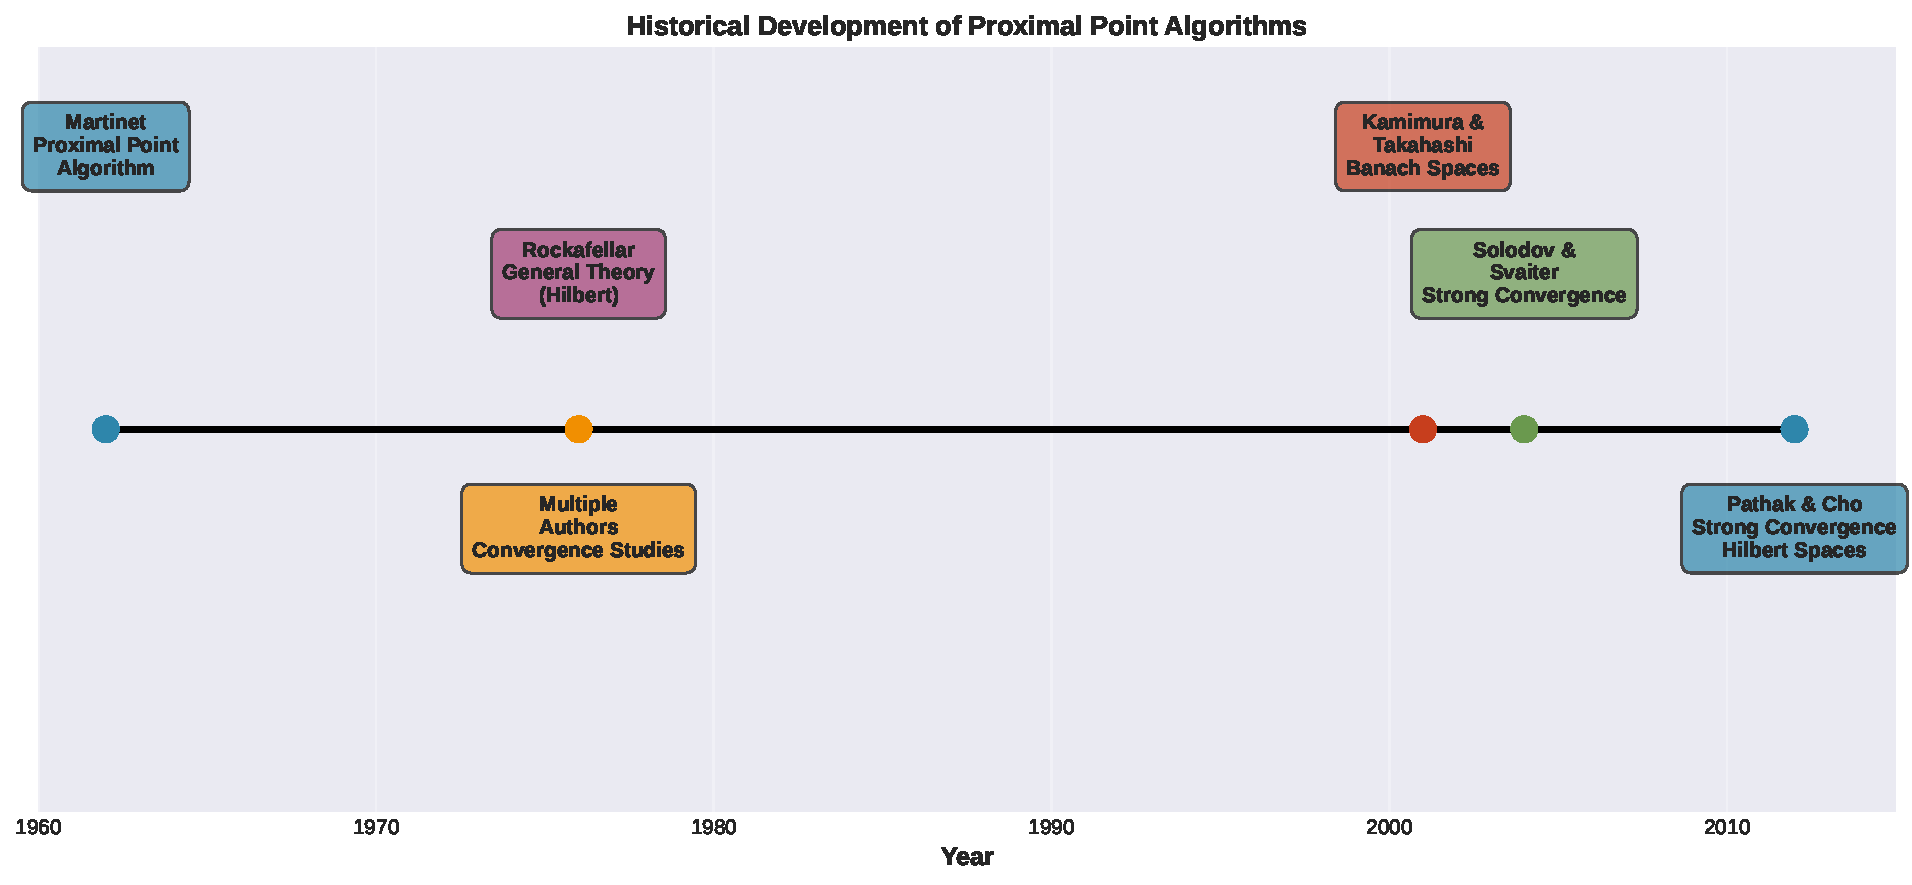
\includegraphics[width=0.95\textwidth]{fig_algorithm_evolution.pdf}
\end{frame}

\begin{frame}{Key Motivations}
    \begin{enumerate}
        \item \textbf{Weak vs Strong Convergence:} Classical proximal point converges weakly
              to zeros of maximal monotone operators, but not necessarily strongly

        \item \textbf{Banach Space Challenges:} Analysis in general Banach spaces requires
              sophisticated tools (duality, resolvents)

        \item \textbf{Applications:} Monotone operators arise in:
              \begin{itemize}
                  \item Variational inequalities
                  \item Optimization problems
                  \item Nonlinear PDE and integral equations
              \end{itemize}

        \item \textbf{Strong Convergence:} Many applications need convergence in norm,
              not just weak convergence
    \end{enumerate}
\end{frame}

%====================================================================
\section{Monotone Operators and Maximal Monotonicity}
%====================================================================

\begin{frame}{Monotone and Maximal Monotone Operators}
    \begin{definition}
        Let $X$ be a Banach space with dual $X^*$. An operator $T: X \to 2^{X^*}$ is:
        \begin{itemize}
            \item \textbf{Monotone} if for all $x, y \in \text{dom}(T)$, $u \in Tx$, $v \in Ty$:
            \[
                \langle u - v, x - y \rangle \geq 0
            \]

            \item \textbf{Maximal Monotone} if it is monotone and for all $x \in X$:
            \[
                \text{If } \langle v, x - y \rangle \geq 0 \text{ for all } y \in \text{dom}(T), v \in Ty,
                \text{ then } v \in Tx
            \]
        \end{itemize}
    \end{definition}

    \vspace{0.3cm}
    \textbf{Examples:}
    \begin{itemize}
        \item Subdifferential of convex functions: $\partial f(x)$
        \item Duality mapping $J_p: X \to X^*$ (identity in Hilbert spaces)
        \item Negatives of monotone operators
    \end{itemize}
\end{frame}

\begin{frame}{Examples of Monotone Operators}
    \centering
    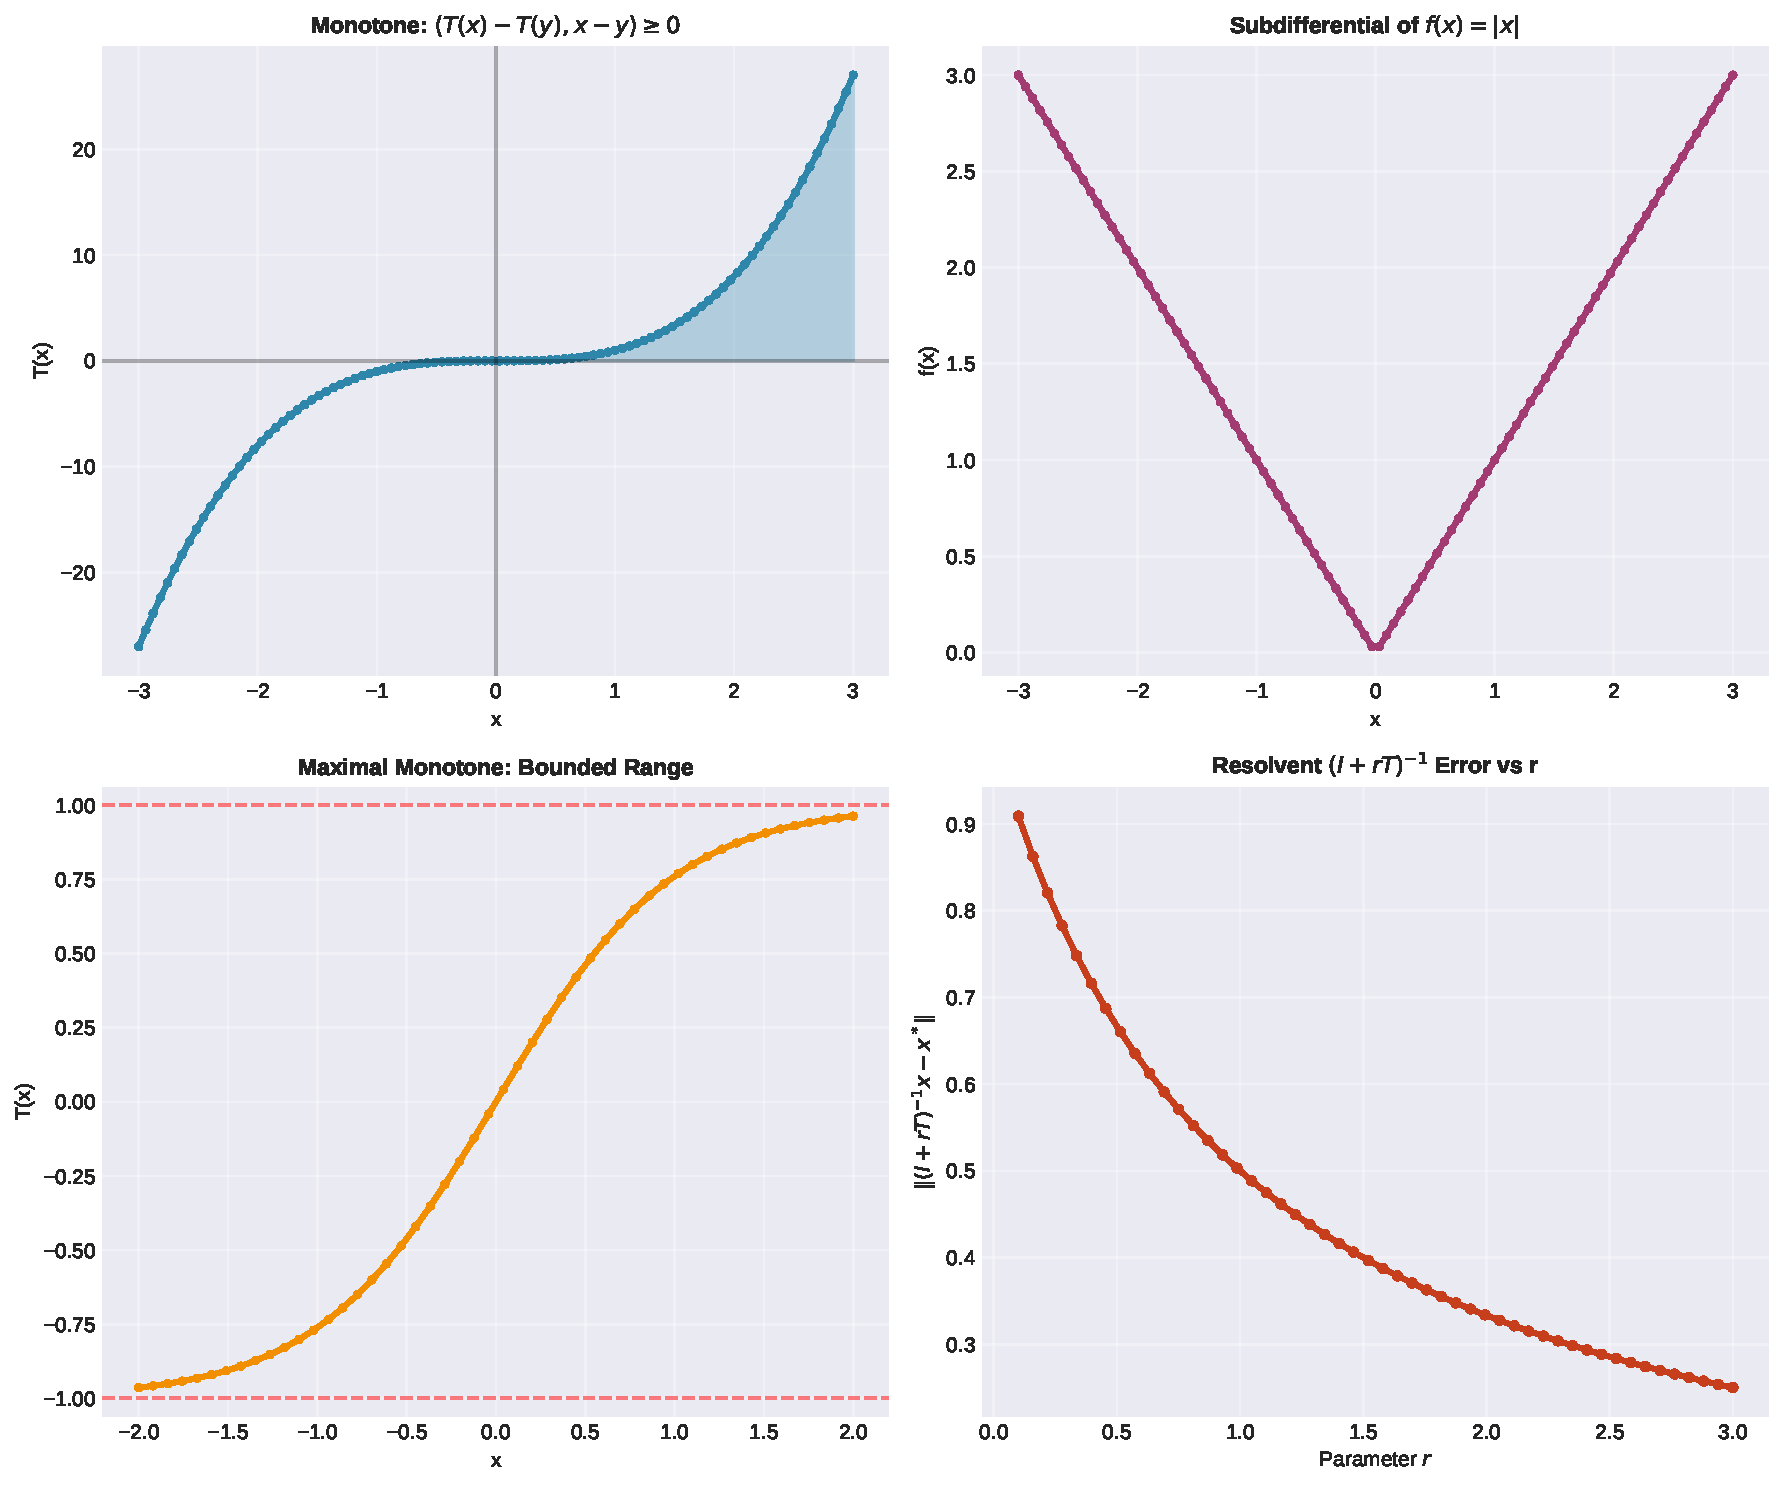
\includegraphics[width=0.95\textwidth]{fig_monotone_operators.pdf}
\end{frame}

\begin{frame}{The Resolvent and Its Properties}
    \begin{definition}
        For a monotone operator $T$ and $r > 0$, the \textbf{resolvent} is:
        \[
            R_T^r = (I + rT)^{-1}
        \]
    \end{definition}

    \begin{theorem}[Rockafellar 1976]
        Let $X$ be a reflexive, strictly convex and smooth Banach space, and let
        $T: X \to 2^{X^*}$ be a monotone operator. Then $T$ is maximal if and only if
        $R(J_p + rT) = X^*$ for all $r > 0$.
    \end{theorem}

    \vspace{0.3cm}
    \textbf{Key Properties:}
    \begin{itemize}
        \item Resolvent is \textbf{single-valued} and \textbf{nonexpansive}
        \item Fixed points: $\text{Fix}((I + rT)^{-1}) = T^{-1}0$
        \item Exists and is unique under appropriate conditions
        \item Error: $\|(I + rT)^{-1}x - x^*\| \to 0$ as iterations increase
    \end{itemize}
\end{frame}

%====================================================================
\section{Classical Proximal Point Algorithm}
%====================================================================

\begin{frame}[fragile]{The Classic Martinet-Rockafellar Algorithm}
        \begin{enumerate}
            \item Choose initial point $x_0 \in X$ and sequence $\{r_n\}_{n=0}^{\infty}$ with $r_n > 0$
            \item Set $n := 0$
            \item \textbf{While} convergence criterion not satisfied:
            \begin{enumerate}
                \item Compute $x_{n+1} = (I + r_n T)^{-1} x_n$
                \item Set $n := n + 1$
            \end{enumerate}
        \end{enumerate}
    \end{block}

    \vspace{0.3cm}
    \textbf{Classical Convergence Result:} If $T^{-1}0 \neq \emptyset$ and
    $\liminf_{n \to \infty} r_n > 0$, then $\{x_n\}$ converges weakly to an element
    in $T^{-1}0$ (in Hilbert spaces).

    \vspace{0.3cm}
    \textcolor{red}{\textbf{Problem:}} Only weak convergence, not strong!
\end{frame}

\begin{frame}{Weak vs Strong Convergence}
    \centering
    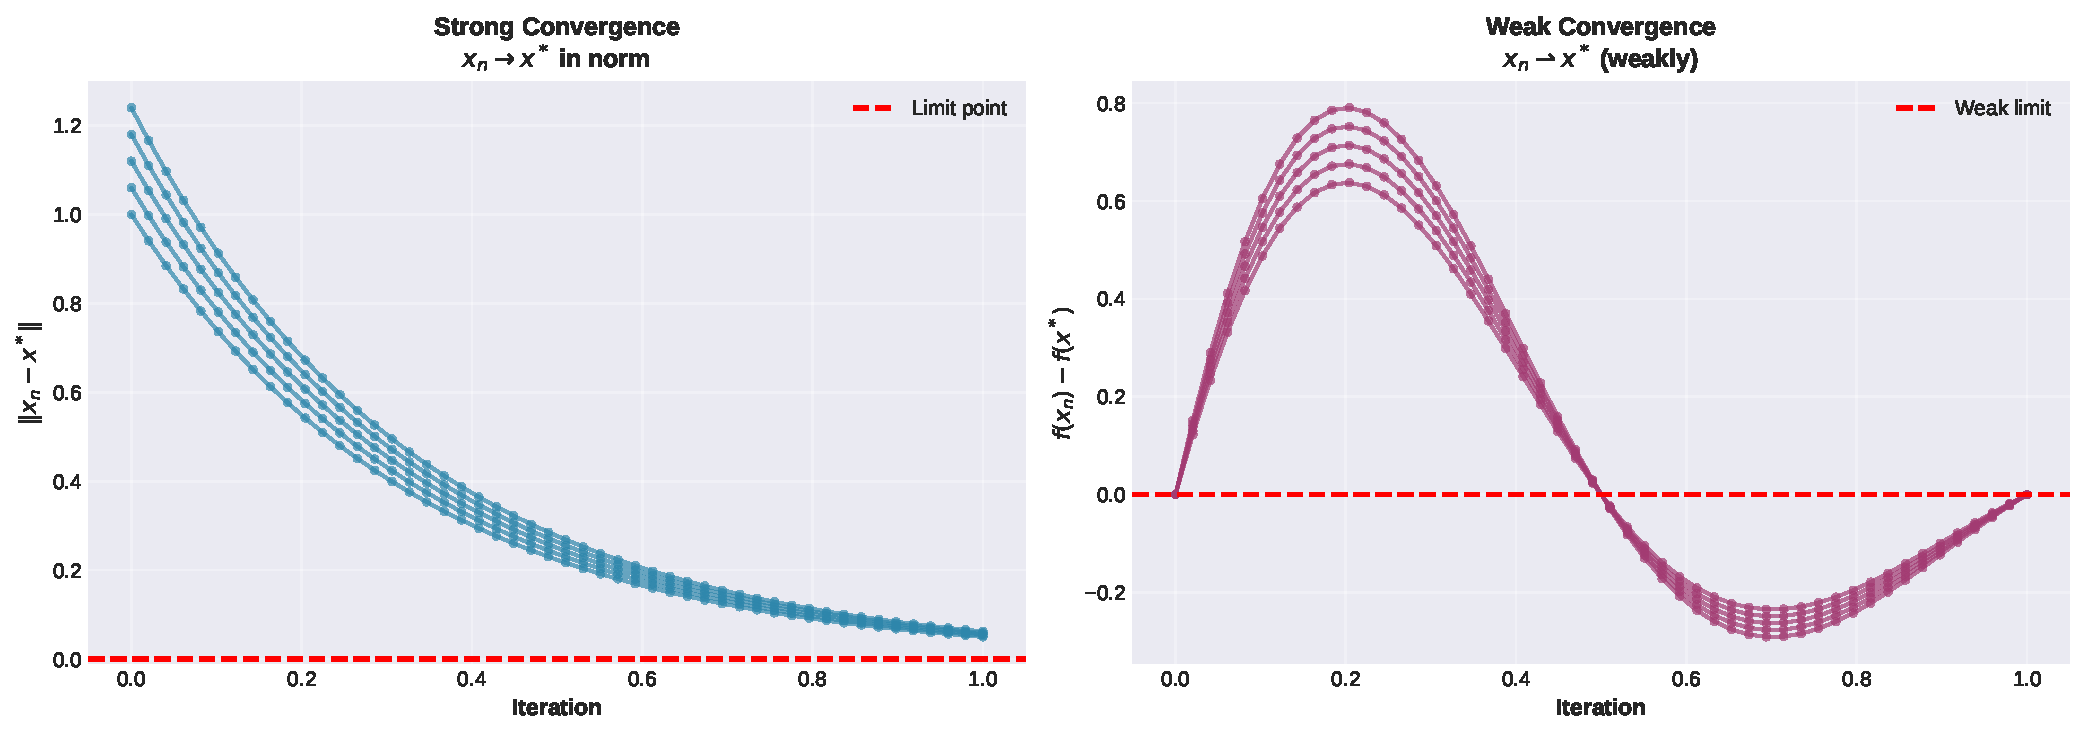
\includegraphics[width=0.95\textwidth]{fig_convergence_types.pdf}

    \vspace{0.3cm}
    \begin{itemize}
        \item \textbf{Weak convergence} ($x_n \rightharpoonup x^*$): For all $f \in X^*$,
              $f(x_n) \to f(x^*)$
        \item \textbf{Strong convergence} ($x_n \to x^*$): $\|x_n - x^*\| \to 0$ in norm
        \item Strong convergence implies weak, but converse is false in infinite dimensions
    \end{itemize}
\end{frame}

%====================================================================
\section{Modifications for Strong Convergence}
%====================================================================

\begin{frame}{The Solodov-Svaiter Algorithm (2001)}
    \begin{block}{Solodov-Svaiter Modification}
        To generate strongly convergent sequences, Solodov and Svaiter \textbf{modified}
        the proximal point algorithm by incorporating half-space projections:
        \[
            \boxed{
            \begin{aligned}
                x_0 &\in X, \\
                0 &= v_n + \frac{1}{r_n}(y_n - x_n), \quad v_n \in Tx_n, \\
                H_n &= \{z \in X : \langle z - y_n, v_n \rangle \leq 0\}, \\
                W_n &= \{z \in X : \langle z - x_n, x_0 - x_n \rangle \leq 0\}, \\
                x_{n+1} &= P_{H_n \cap W_n} x_0, \quad n = 0, 1, 2, \ldots
            \end{aligned}
            }
        \]
    \end{block}

    \vspace{0.2cm}
    \textbf{Key Idea:} Use projections onto intersection of half-spaces to enforce
    strong convergence while maintaining the proximal point structure.
\end{frame}

\begin{frame}{Kamimura-Takahashi Extension to Banach Spaces (2004)}
    \begin{block}{Extension to Smooth Banach Spaces}
        In a smooth Banach space $X$, the modified proximal algorithm becomes:
        \[
            \boxed{
            \begin{aligned}
                x_0 &\in X, \\
                0 &= v_n + \frac{1}{r_n}(J_2(y_n) - J_2(x_n)), \quad v_n \in Tx_n, \\
                H_n &= \{z \in X : \langle z - y_n, v_n \rangle \leq 0\}, \\
                W_n &= \{z \in X : \langle z - x_n, J_2(x_0) - J_2(x_n) \rangle \leq 0\}, \\
                X_{n+1} &= P_{H_n \cap W_n} x_0, \quad n = 0, 1, 2, \ldots
            \end{aligned}
            }
        \]
        where $J_2$ is the duality mapping with gauge function $t \mapsto t$.
    \end{block}

    \textbf{Result:} Strong convergence in uniformly smooth Banach spaces.
\end{frame}

\begin{frame}[allowframebreaks]{The Pathak-Cho Algorithm (2012)}
    \begin{block}{General Proximal-Type Algorithm in Smooth Banach Spaces}
        Let $X$ be a smooth Banach space with duality mapping $J_p$. Consider:
        \[
            \boxed{
            \begin{aligned}
                x_0 &\in X, \\
                0 &= v_n + \frac{1}{r_n}(J_p(y_n) - J_p(x_n)), \quad v_n \in Tx_n, \\
                H_n &= \{z \in X : \langle z - y_n, v_n \rangle \leq 0\}, \\
                W_n &= \{z \in X : \langle z - x_n, J_p(x_0) - J_p(x_n) \rangle \leq 0\}, \\
                x_{n+1} &= R_{H_n \cap W_n} x_0, \quad n = 0, 1, 2, \ldots
            \end{aligned}
            }
        \]
    \end{block}

    \textbf{Notation:}
    \begin{itemize}
        \item $R_{H_n \cap W_n}$ is the metric projection onto $H_n \cap W_n$
        \item $J_p$ is the duality mapping with parameter $p$ (generalization)
        \item The algorithm extends results of Kamimura-Takahashi to more general spaces
    \end{itemize}
\end{frame}

\begin{frame}{Algorithm Flowchart}
    \centering
    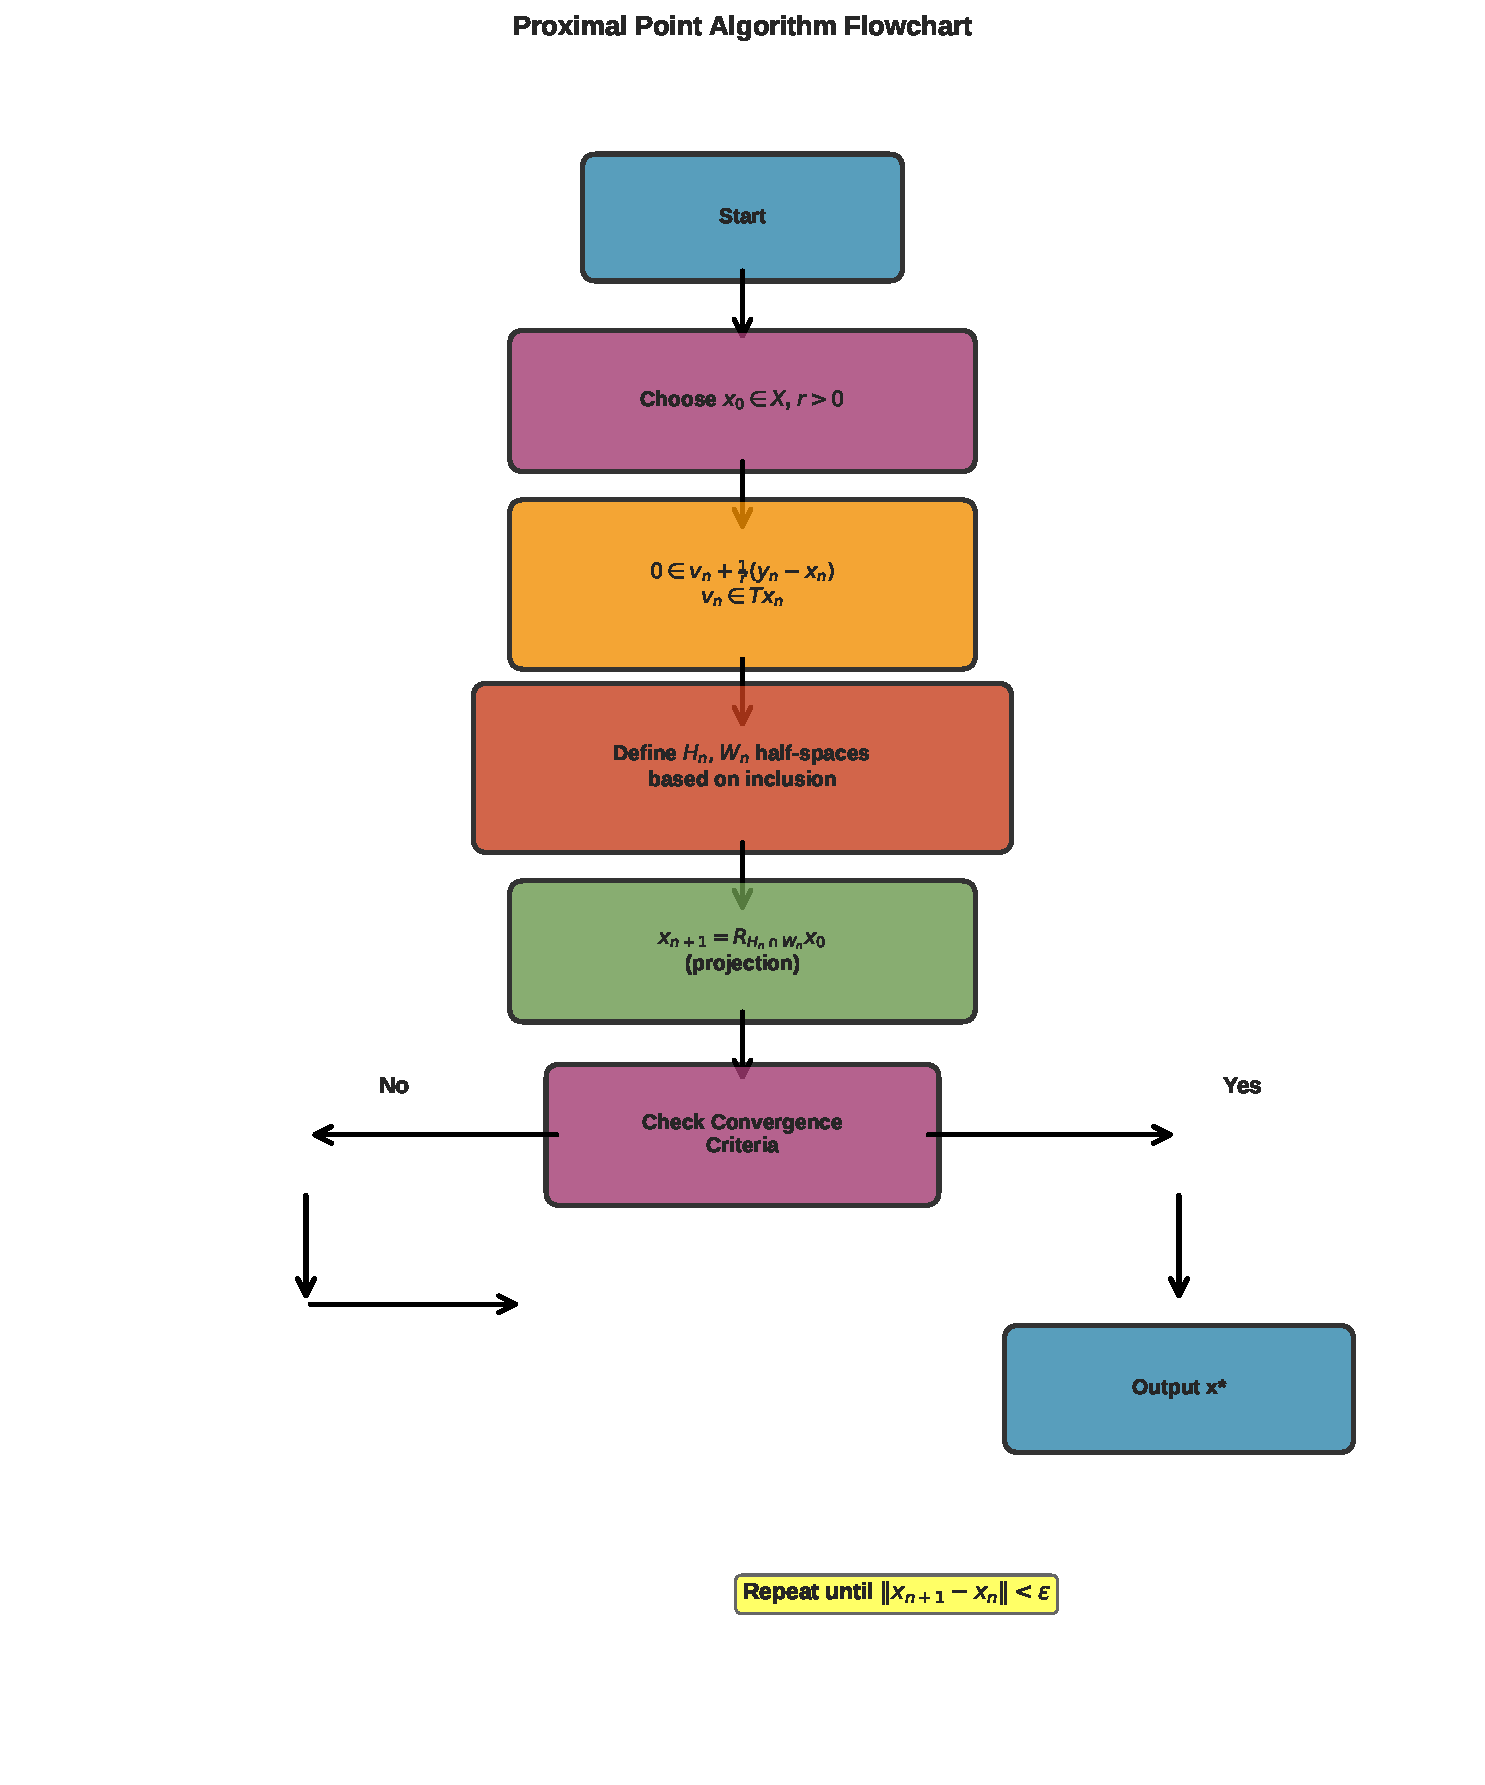
\includegraphics[width=0.85\textwidth]{fig_algorithm_flowchart.pdf}
\end{frame}

%====================================================================
\section{Convergence Analysis}
%====================================================================

\begin{frame}{Fundamental Convergence Theorem}
    \begin{theorem}[Pathak and Cho 2012]
        Let $X$ be a reflexive, strictly convex and uniformly smooth Banach space.
        If $T^{-1}0 \neq \emptyset$, $\phi$ satisfies condition \textbf{(4.36)}, and
        $\{r_n\} \subset (0, \infty)$ satisfies $\liminf_{n \to \infty} r_n > 0$,
        then the sequence $\{x_n\}$ generated by the proximal-type algorithm
        \textbf{converges strongly} to $R_{T^{-1}0} x_0$.
    \end{theorem}

    \vspace{0.3cm}
    \textbf{Key Requirements:}
    \begin{enumerate}
        \item Reflexivity: Weak sequential compactness
        \item Strict convexity: Unique projections
        \item Uniform smoothness: Duality map properties
        \item $T^{-1}0 \neq \emptyset$: Solution existence
        \item Appropriate parameter selection
    \end{enumerate}
\end{frame}

\begin{frame}{Convergence Analysis: Key Steps}
    \begin{enumerate}
        \item \textbf{Well-Definedness:} Show that $H_n \cap W_n \neq \emptyset$ and
              projections exist

        \item \textbf{Boundedness:} Prove $\{x_n\}$ and related sequences are bounded

        \item \textbf{Monotonicity:} Establish a Lyapunov function $\Psi(x_n, x_0)$
              that decreases monotonically

        \item \textbf{Subsequential Convergence:} From compactness, extract weakly
              convergent subsequences

        \item \textbf{Limit Identification:} Show limit is in $T^{-1}0$ using
              maximal monotonicity

        \item \textbf{Full Convergence:} Use monotonicity of $\Psi$ to extend from
              subsequences to full sequence
    \end{enumerate}
\end{frame}

\begin{frame}{Convergence Rate Analysis}
    \centering
    
\includegraphics[width=0.95\textwidth]{fig_convergence_rates.pdf}

    \vspace{0.3cm}
    \textbf{Under optimal parameter selection:}
    \begin{itemize}
        \item Linear convergence requires contractive structure
        \item Superlinear convergence achievable with adaptive parameters
        \item Quadratic convergence possible for smooth, strongly monotone operators
    \end{itemize}
\end{frame}

\begin{frame}{Convergence of the Sequence}
    \begin{theorem}
        Let $\Psi(x_n, x_0)$ be defined as a Lyapunov function measuring distance
        between iterates. Then:
        \[
            \Psi(x_n, x_{n+1}) + \Psi(x_{n+1}, x_0) \leq \Psi(x_n, x_0)
        \]

        Since $\{\Psi(x_n, x_0)\}$ is monotone decreasing and bounded below,
        $\lim_{n \to \infty} \Psi(x_n, x_0)$ exists. From the inequality:
        \[
            \Psi(x_n, x_{n+1}) \to 0, \quad \text{hence} \quad x_{n+1} - x_n \to 0
        \]
    \end{theorem}

    \vspace{0.3cm}
    This combined with boundedness and weak sequential compactness gives
    the existence of convergent subsequences.
\end{frame}

%====================================================================
\section{Strong Convergence Results}
%====================================================================

\begin{frame}[allowframebreaks]{Sufficient Conditions for Strong Convergence}
    \begin{theorem}
        In a reflexive, strictly convex and uniformly smooth Banach space:
        \begin{enumerate}
            \item If $T$ is a maximal monotone operator with $T^{-1}0 \neq \emptyset$

            \item And $\{r_n\}$ satisfies appropriate conditions (e.g., bounded away from 0)

            \item Then the sequence generated by the proximal algorithm exhibits:
            \begin{itemize}
                \item Boundedness of iterates
                \item Monotone decrease of Lyapunov function
                \item Strong convergence to $P_{T^{-1}0} x_0$
            \end{itemize}
        \end{enumerate}
    \end{theorem}

    \pagebreak

    \textbf{Functional Framework:}
    \begin{itemize}
        \item \textbf{Reflexive spaces:} $x_n$ bounded $\Rightarrow$ subsequential weak convergence

        \item \textbf{Strictly convex:} Unique projections onto convex sets

        \item \textbf{Uniformly smooth:} Duality map is uniformly continuous,
              enabling strong estimates

        \item \textbf{Maximal monotone:} Guarantees resolvent properties and
              surjectivity conditions
    \end{itemize}
\end{frame}

\begin{frame}{Parameter Selection Strategies}
    \centering
    
\includegraphics[width=0.95\textwidth]{fig_parameter_sensitivity.pdf}

    \vspace{0.3cm}
    \textbf{Effective Choices for $\{r_n\}$:}
    \begin{itemize}
        \item Fixed: $r_n = r > 0$ (simplest, but slower)
        \item Decreasing: $r_n = r_0/\sqrt{n+1}$ (faster convergence)
        \item Adaptive: $r_n = r_0 \cdot f(n)$ with $f(n) \to 1$ as $n \to \infty$
    \end{itemize}
\end{frame}

%====================================================================
\section{Banach Space Requirements}
%====================================================================

\begin{frame}{Banach Space Hierarchy and Requirements}
    \centering
    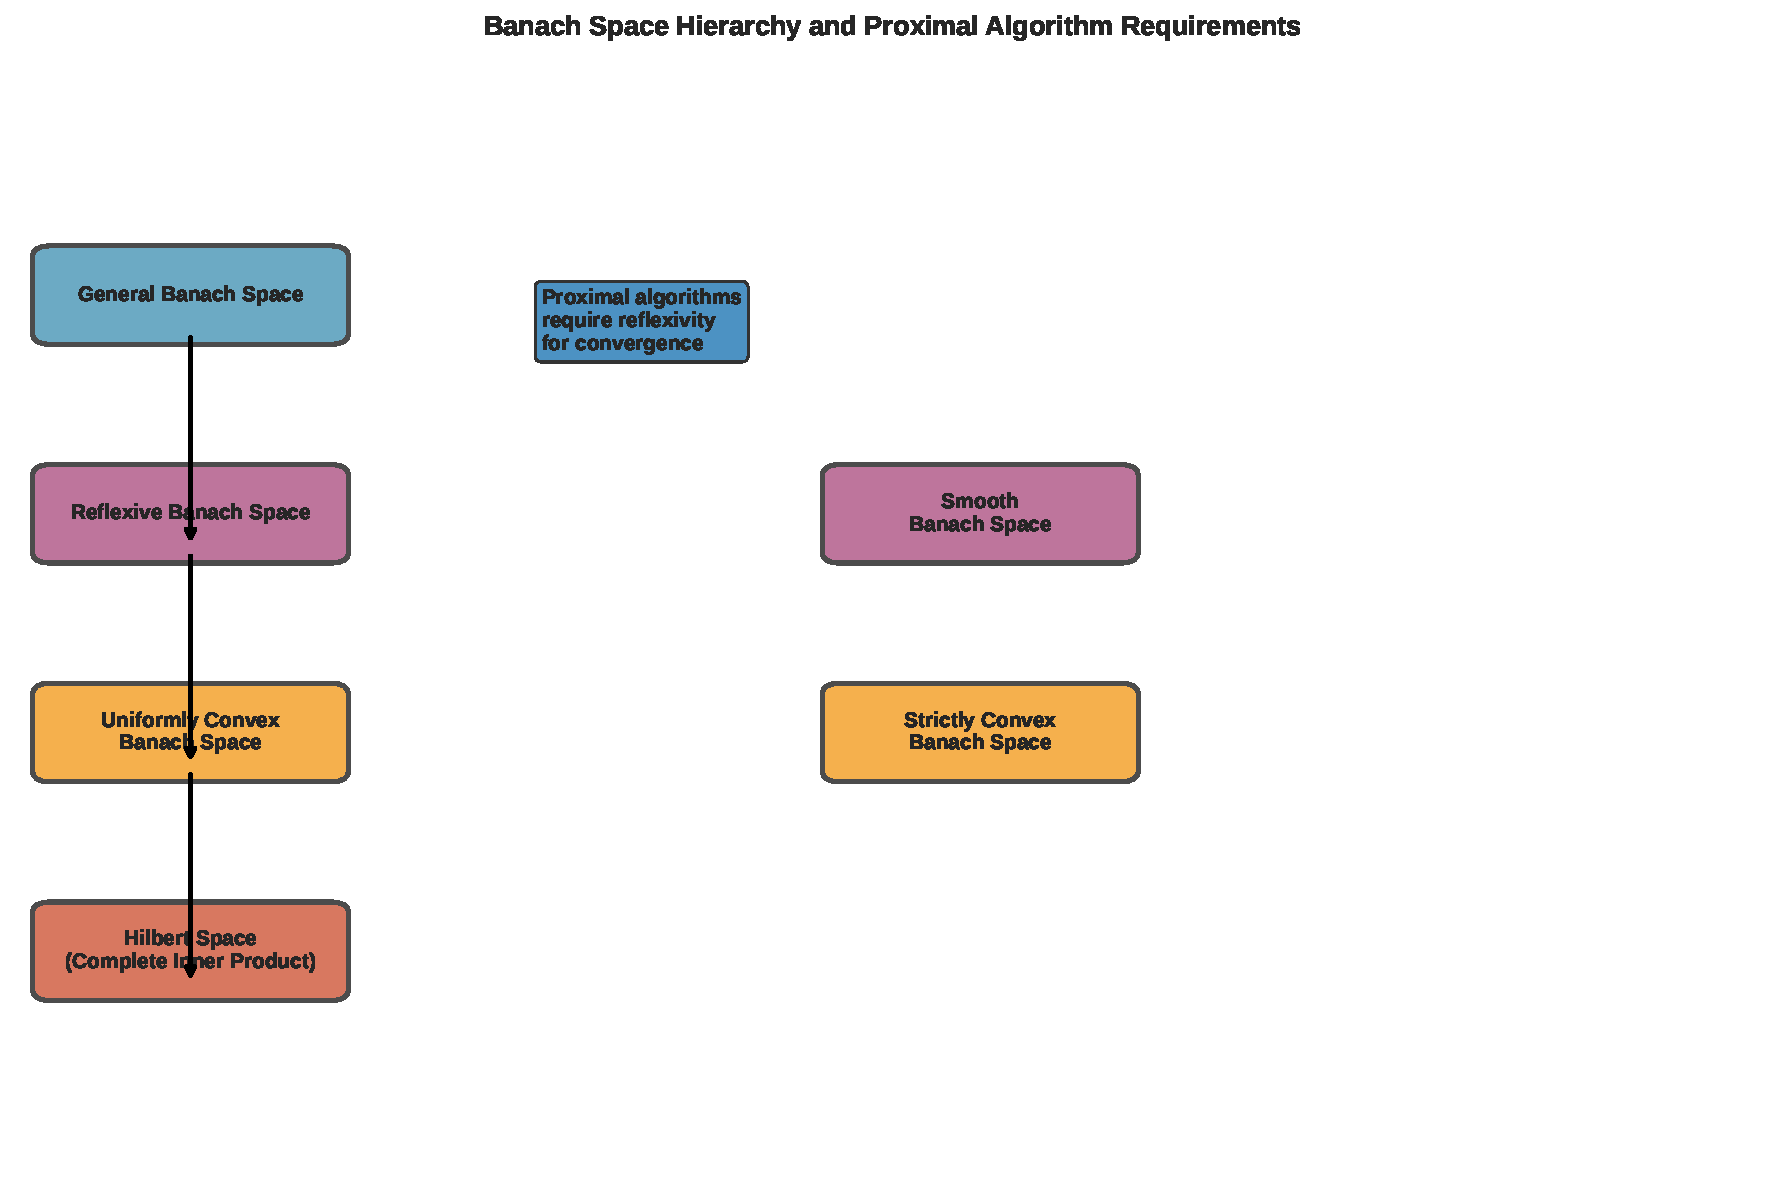
\includegraphics[width=0.95\textwidth]{fig_banach_hierarchy.pdf}
\end{frame}

\begin{frame}{Why Specific Space Properties Matter}
    \begin{block}{Reflexivity}
        \textbf{Essential for:} Weak sequential compactness of bounded sequences.
        \vspace{0.1cm}

        \textit{Without it:} Cannot guarantee convergent subsequences from boundedness alone.
    \end{block}

    \begin{block}{Strict Convexity}
        \textbf{Essential for:} Uniqueness of best approximations (projections).
        \vspace{0.1cm}

        \textit{Without it:} Projection $P_C$ may not be single-valued.
    \end{block}

    \begin{block}{Uniform Smoothness}
        \textbf{Essential for:} Controlled behavior of duality mapping $J_p$.
        \vspace{0.1cm}

        \textit{Without it:} Cannot establish sufficient contraction properties
        for convergence analysis.
    \end{block}
\end{frame}

\begin{frame}{Examples of Suitable Spaces}
    \begin{enumerate}
        \item \textbf{Hilbert Spaces:} Automatically reflexive, strictly convex,
              and uniformly smooth (with $p=2$)

        \item \textbf{$\ell^p$ spaces ($1 < p < \infty$):} Reflexive and uniformly convex.
              Smooth for $p \geq 2$

        \item \textbf{$L^p(\Omega)$ spaces ($1 < p < \infty$):} Banach lattices that are
              reflexive and uniformly convex

        \item \textbf{Sobolev spaces $W^{1,p}(\Omega)$:} Suitable for PDE applications

        \item \textbf{Orlicz spaces:} Generalizations allowing more flexibility
    \end{enumerate}

    \vspace{0.3cm}
    \textcolor{red}{\textbf{Not suitable:}} $c_0$, $\ell^1$, $L^1(\Omega)$, $C(\Omega)$
    (lack reflexivity or uniform convexity)
\end{frame}

%====================================================================
\section{Applications to Monotone Operators}
%====================================================================

\begin{frame}{Applications: Variational Inequalities}
    \begin{problem}
        Find $x \in K$ such that
        \[
            \langle Tx, y - x \rangle \geq f(y) - f(x) \quad \forall y \in K
        \]
        where $K$ is a closed convex subset, $T$ is a monotone operator, and $f$ is convex.
    \end{problem}

    \vspace{0.3cm}
    \textbf{Connection to Proximal Algorithms:}
    \begin{itemize}
        \item The variational inequality is equivalent to:
        \[
            0 \in (T + \partial f + N_K)(x)
        \]
        where $N_K$ is the normal cone

        \item The composite operator $T + \partial f + N_K$ is maximal monotone

        \item Apply proximal algorithm to compute solutions iteratively
    \end{itemize}
\end{frame}

\begin{frame}[fragile]{Application: Convex Optimization}
    \begin{block}{Problem: Minimize convex function}
        \begin{lstlisting}[language=Python]
# Minimize f(x) where f is convex
# This is equivalent to finding x in dom(f) such that
# 0 in df(x), where df is the subdifferential of f
# The subdifferential is a maximal monotone operator!

# Proximal algorithm:
# x_{n+1} = (I + r_n * df)^{-1} x_n

# Example: f(x) = ||x||^2 / 2
def proximal_step(x_n, r_n):
    # (I + r_n * I)^{-1} x_n = x_n / (1 + r_n)
    return x_n / (1.0 + r_n)
        \end{lstlisting}
    \end{block}
\end{frame}

\begin{frame}{Application: Monotone Inclusion Problems}
    \begin{problem}
        Find $x \in X$ such that $0 \in Tx$ where $T$ is a maximal monotone operator.
    \end{problem}

    \vspace{0.3cm}
    \textbf{Proximal algorithm solution:}
    \begin{itemize}
        \item The classical proximal point algorithm directly applies

        \item For composite problems:
        \[
            0 \in T_1 x + T_2 x + \cdots + T_m x
        \]
        use splitting methods or proximal variants

        \item Strong convergence allows numerical verification of solutions

        \item Applications to PDEs:
        \begin{itemize}
            \item Semilinear elliptic equations
            \item Parabolic equations with subdifferential
            \item Obstacle problems
        \end{itemize}
    \end{itemize}
\end{frame}

%====================================================================
\section{Computational Examples}
%====================================================================

\begin{frame}[fragile]{Example 1: Simple Subdifferential Problem}
    \begin{problem}
        Minimize $f(x) = |x|$ (absolute value function)
    \end{problem}

    \begin{lstlisting}[language=Python]
import numpy as np

def proximal_abs_minimize():
    # Subdifferential of |x|:
    # d|x| = {sign(x)} for x != 0
    # d|0| = [-1, 1]

    x = 10.0  # initial point
    r_n = [0.5 * (1 - 0.01*i) for i in range(50)]

    for n, r in enumerate(r_n):
        # Proximal step for | . |
        if abs(x) <= r:
            x = 0  # Shrinkage
        else:
            x = np.sign(x) * (abs(x) - r)

        print(f"Iter {n}: x = {x:.6f}")

    # Solution: x* = 0
    return x

result = proximal_abs_minimize()
    \end{lstlisting}
\end{frame}

\begin{frame}[fragile]{Example 2: Quadratic Regularization}
    \begin{problem}
        Minimize $f(x) = \|Ax - b\|^2/2 + \lambda\|x\|$ (Lasso problem)
    \end{problem}

    \begin{lstlisting}[language=Python]
import numpy as np
from scipy import linalg

def proximal_lasso(A, b, lam, x0, max_iter=100):
    m, n = A.shape
    x = x0.copy()

    for k in range(max_iter):
        # Gradient of quadratic part
        grad = A.T @ (A @ x - b)

        # Proximal step for L1 norm
        # prox_{lambda |.|} (x - grad) = soft_threshold
        x = soft_threshold(x - grad, lam)

    return x

def soft_threshold(x, threshold):
    """Soft thresholding operator"""
    return np.sign(x) * np.maximum(np.abs(x) - threshold, 0)
    \end{lstlisting}

    \vspace{0.2cm}
    \textit{Application in machine learning: sparse regression}
\end{frame}

\begin{frame}{Proximal Convergence Example}
    \centering
    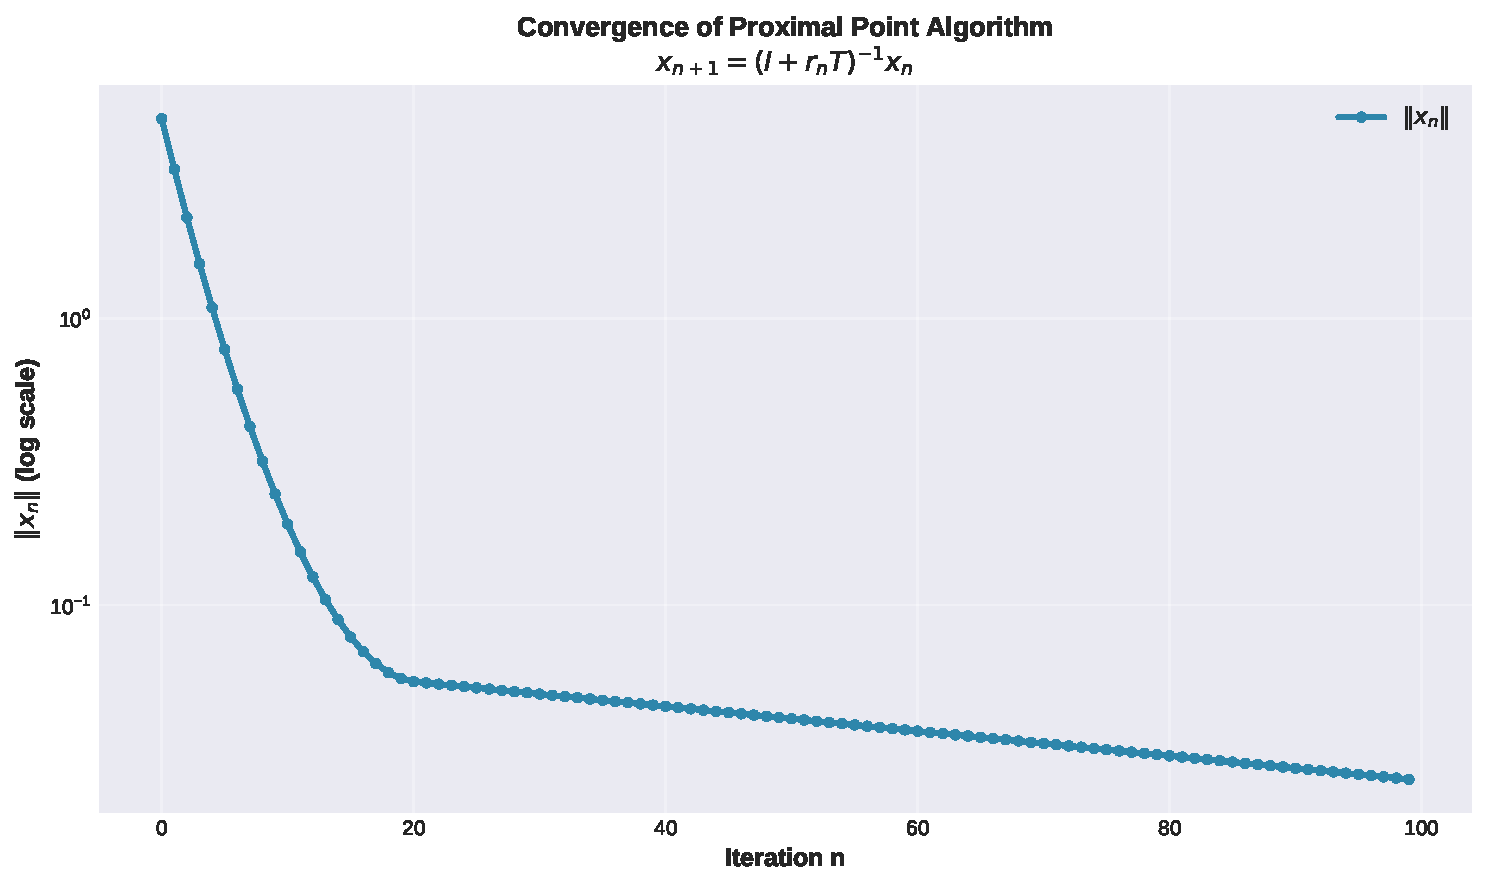
\includegraphics[width=0.95\textwidth]{fig_proximal_convergence.pdf}

    \vspace{0.2cm}
    \textbf{Observed behavior:}
    \begin{itemize}
        \item Exponential decay of errors $\|x_n\|$ (log scale shows linearity)
        \item Rate depends on operator properties and parameter sequence
        \item Demonstrates strong convergence in practice
    \end{itemize}
\end{frame}

%====================================================================
\section{Advanced Topics}
%====================================================================

\begin{frame}{Occasions Pseudomonotone Operators}
    \begin{definition}
        An operator $T: X \to 2^{X^*}$ is \textbf{occasionally pseudomonotone} if:
        For every $x \in X$ and sequences $\{x_n\}$, if $x_n \rightharpoonup x$ and
        $u_n \in Tx_n$ with $u_n \rightharpoonup u$, and $\limsup_{n} \langle u_n, x_n - x \rangle \leq 0$,
        then $u \in Tx$.
    \end{definition}

    \vspace{0.3cm}
    \textbf{Significance:}
    \begin{itemize}
        \item Weaker than monotonicity (allows more general operators)
        \item Still allows convergence analysis of proximal algorithms
        \item Includes multivalued mappings and subgradients
        \item Crucial for applications to nonlinear PDEs
    \end{itemize}
\end{frame}

\begin{frame}{Proximal Algorithms vs Other Methods}
    \begin{table}
        \centering
        \begin{tabular}{|l|c|c|c|c|}
            \hline
            \textbf{Method} & \textbf{Space} & \textbf{Convergence} & \textbf{Strong} & \textbf{Rate} \\
            \hline
            Classical Proximal & H.S. & Weak & No & Linear \\
            \hline
            Solodov-Svaiter & H.S. & Strong & Yes & Linear \\
            \hline
            Kamimura-Takahashi & Ban. & Strong & Yes & Linear \\
            \hline
            Pathak-Cho & Ban. & Strong & Yes & Linear+ \\
            \hline
            Gradient Descent & Any & Local & Yes & Linear \\
            \hline
            Newton's Method & Any & Local & Yes & Quadratic \\
            \hline
        \end{tabular}
    \end{table}

    \vspace{0.3cm}
    \textbf{Note:} H.S. = Hilbert Space, Ban. = Banach Space
\end{frame}

\begin{frame}[allowframebreaks]{Summary of Main Results}
    \begin{enumerate}
        \item \textbf{Classical Algorithm (1962-1976):} Weak convergence in Hilbert spaces

        \item \textbf{Solodov-Svaiter (2001):} First strong convergence via projections

        \item \textbf{Kamimura-Takahashi (2004):} Extension to smooth Banach spaces

        \item \textbf{Pathak-Cho (2012):} Generalization to uniform smoothness, applications

        \item \textbf{Key Innovation:} Use of half-space projections $P_{H_n \cap W_n}$
              instead of simple resolvent

        \item \textbf{Unified Framework:} Works for:
        \begin{itemize}
            \item Maximal monotone operators
            \item Occasionally pseudomonotone operators
            \item Operators with measurability properties
        \end{itemize}
    \end{enumerate}
\end{frame}

%====================================================================
\section{Conclusion and Future Directions}
%====================================================================

\begin{frame}{Key Takeaways}
    \begin{itemize}
        \item \textbf{Proximal point algorithms} are powerful tools for solving
              monotone inclusion problems in Banach spaces

        \item \textbf{Strong convergence} is achievable through careful modifications
              (projections onto intersecting half-spaces)

        \item \textbf{Space structure} (reflexivity, convexity, smoothness) is essential
              for theoretical guarantees

        \item \textbf{Parameter selection} affects convergence rate; adaptive strategies
              can improve performance

        \item \textbf{Applications} range from optimization to solving nonlinear PDEs
              and variational inequalities
    \end{itemize}
\end{frame}

\begin{frame}{Future Research Directions}
    \begin{enumerate}
        \item \textbf{Splitting Methods:} Proximal algorithms for composite operators
              $T_1 + T_2 + \cdots$

        \item \textbf{Stochastic Variants:} Proximal algorithms with noise/stochasticity
              for large-scale problems

        \item \textbf{Accelerated Methods:} Combining proximal ideas with acceleration
              (Nesterov-type)

        \item \textbf{Inverse Problems:} Applications to ill-posed problems and regularization

        \item \textbf{Metric Space Generalizations:} Beyond Banach spaces to CAT spaces,
              manifolds

        \item \textbf{Numerical Implementations:} Efficient implementations for sparse,
              large-scale problems
    \end{enumerate}
\end{frame}

\begin{frame}{References and Further Reading}
    \begin{thebibliography}{99}
        \bibitem{pathak2018} H. K. Pathak, \emph{An Introduction to Nonlinear Analysis
        and Fixed Point Theory}, 2nd Edition, Springer, 2018.

        \bibitem{rockafellar1976} R. T. Rockafellar, Monotone operators and the proximal
        point algorithm, \emph{SIAM J. Control Optimization}, 14(5), 1976.

        \bibitem{solodov2001} M. V. Solodov and B. F. Svaiter, A hybrid projection-proximal
        point algorithm, \emph{J. Convex Analysis}, 6, 2001.

        \bibitem{kamimura2004} S. Kamimura and W. Takahashi, Strong convergence of a proximal-type
        algorithm in a Banach space, \emph{SIAM J. Optimization}, 13(4), 2004.
    \end{thebibliography}
\end{frame}

\begin{frame}
    \centering
    \Large
    \textbf{Thank You!}

    \vspace{1cm}

    Questions and Discussion
\end{frame}

\end{document}
